% Created 2014-05-28 Wed 12:26
\documentclass[t]{beamer}
\usepackage[utf8]{inputenc}
\usepackage[T1]{fontenc}
\usepackage{fixltx2e}
\usepackage{graphicx}
\usepackage{longtable}
\usepackage{float}
\usepackage{wrapfig}
\usepackage{soul}
\usepackage{textcomp}
\usepackage{marvosym}
\usepackage{wasysym}
\usepackage{latexsym}
\usepackage{amssymb}
\usepackage{hyperref}
\tolerance=1000
\mode<beamer>{\usetheme{TUD}}
\usepackage{tikz}
\usetikzlibrary{positioning,chains,arrows,shadows,fadings,shapes,backgrounds,snakes,matrix,patterns,plotmarks,trees,mindmap}
\usepackage[absolute,overlay]{textpos}
\usepackage{pgfpages} 
\graphicspath{{./}{figs/}{figures/}{../logos/}{../cfigures/}{../RTS-2011/figs/}{}}
\newcommand{\floor}[1]{\left\lfloor{#1}\right\rfloor}
\newcommand{\setof}[1]{\left\{{#1}\right\}}
\newcommand{\set}[2]{\left\{{#1}\mid{#2}\right\}}
\newcommand{\ceiling}[1]{\left\lceil{#1}\right\rceil}
\newcommand{\red}[1]{\textcolor{red}{#1}}
\newcommand{\blue}[1]{\textcolor{blue}{#1}}
\providecommand{\alert}[1]{\textbf{#1}}

\title{Semaphore in RTEMS}
\author{Kuan-Hsun Chen}

\institute{LS 12, TU Dortmund}
\date{04,08,2015}
\hypersetup{
  pdfkeywords={},
  pdfsubject={},
  pdfcreator={Emacs Org-mode version 7.9.3f}}

\tikzset{
    task/.style={shade, shading=radial, rectangle,minimum height=.1cm,
        inner color=#1!20, outer color=#1!60!gray},
    task1/.style={task=yellow, minimum width=13mm},
    task2/.style={task=green, minimum width=13mm},
    task3/.style={task=red, minimum width=13mm},
    task4/.style={task=orange, minimum width=13mm},
    task5/.style={task=blue, minimum width=13mm},
    task6/.style={task=purple, minimum width=13mm},
    task7/.style={task=cyan, minimum width=13mm},
    task8/.style={task=pink, minimum width=13mm},
}

\tikzstyle{circleNode}=[circle,thick,draw=blue!75,fill=blue!20,minimum size=6mm]
\tikzstyle{niceFill}=[thick,draw=blue!75,fill=blue!20,minimum size=6mm]

\begin{document}

\maketitle

\begin{frame}
\frametitle{Outline}

\begin{itemize}

\item Introduction of Semaphore in RTEMS
\label{sec-1-1}%

\item Priority Inversion

\item Priority Inheritance Protocols

\item Exercises 

\end{itemize} % ends low level
\end{frame}

\begin{frame}
\frametitle{Semaphore in RTEMS}
\label{sec-2}
\begin{itemize}

\item Semaphore Attribute Set (Possible combinations)
\begin{center}
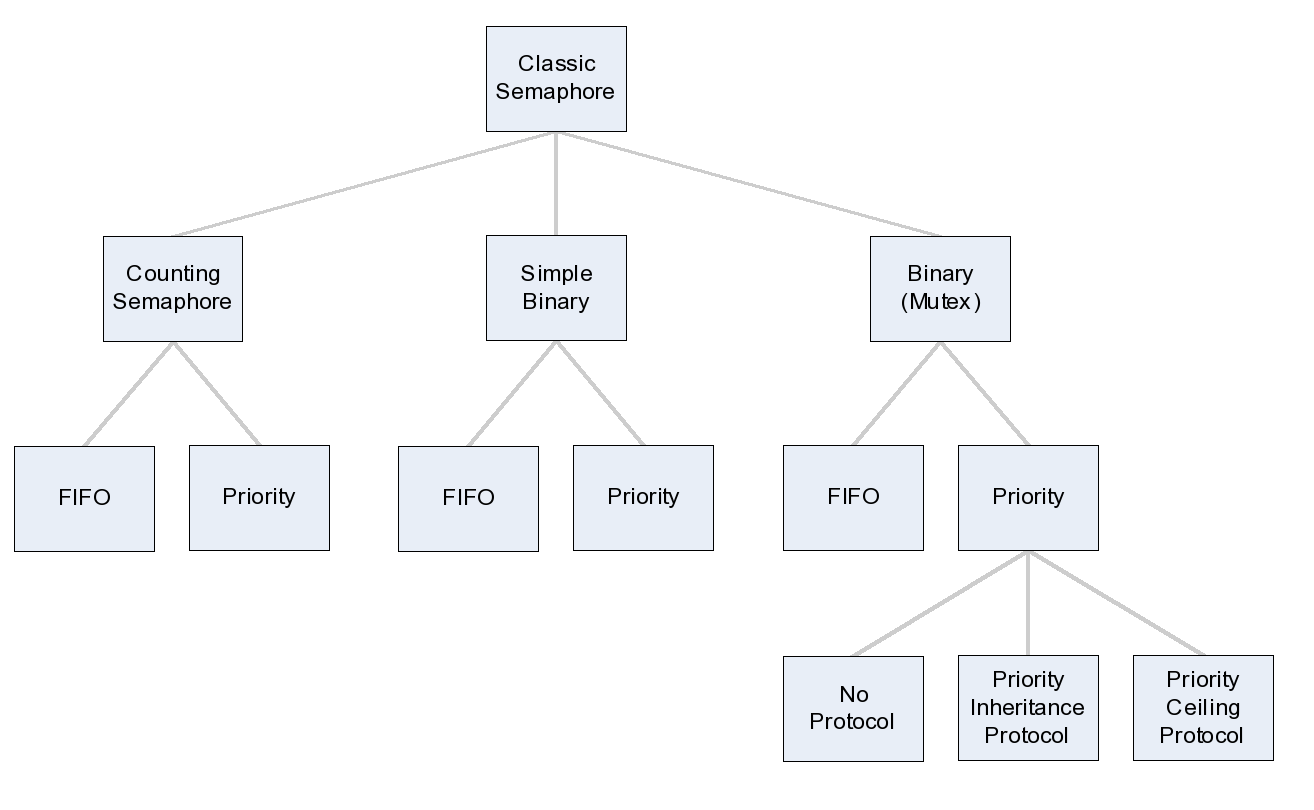
\includegraphics[width=0.9\textwidth]{semaphore_attributes}
\end{center}
\item \scriptsize Source from \url{https://docs.rtems.org/doc-current/share/rtems/html/c_user/Semaphore-Manager-Building-a-Semaphore-Attribute-Set.html}
\end{itemize} % ends low level

\end{frame}

\begin{frame}
\frametitle{Features of RTEMS}
\begin{itemize}
\item rtems\_semaphore\_create(name, count, attribute\_set, priority\_ceiling, rtems\_id *id)
\item Some attributes:
\begin{itemize}

\scriptsize{
\item    RTEMS\_FIFO - tasks wait by FIFO (default)
\item    RTEMS\_PRIORITY - tasks wait by priority
\item    RTEMS\_COUNTING\_SEMAPHORE - no restriction on values (default)
\item    RTEMS\_BINARY\_SEMAPHORE - restrict values to 0 and 1
\item    RTEMS\_NO\_INHERIT\_PRIORITY - do not use priority inheritance (default)
\item    RTEMS\_NO\_PRIORITY\_CEILING - do not use priority ceiling (default)
\item    RTEMS\_LOCAL - local semaphore (default)
\item ...
}
\end{itemize}
\item For example:{ \scriptsize{RTEMS\_BINARY\_SEMAPHORE | RTEMS\_FIFO | RTEMS\_NO\_INHERIT\_PRIORITY | RTEMS\_NO\_PRIORITY\_CEILING | RTEMS\_LOCAL}}
\item Count should be larger than 1 for the normal usage of binary/counting semaphore. 
\end{itemize}
\end{frame}

\begin{frame}
\frametitle{Dig into the source code cpukit/}
\begin{itemize}
\item In fact Binary Semaphore in RTEMS is implemented by the structure of Mutex. (Binary Semaphore != Mutex)
\item RTEMS interface:
\begin{itemize}
\item rtems\_semaphore\_obtain() is implemented into rtems/src/semobtain.c
\item rtems\_semaphore\_release() is implemented into rtems/src/semrelease.c
\end{itemize}
\item Core functions:
\begin{itemize}
\item \_CORE\_mutex\_Seize\_interrupt\_blocking() in score/src/coremutexseize.c
\item \_Thread\_Raise\_priority() in score/src/threadchangepriority.c
\end{itemize}

\end{itemize}
\end{frame}

\begin{frame}
  \frametitle{Priority Inversion}
  
    A higher priority job
    is \emph{blocked} by a lower-priority job.

    \begin{itemize}
    \item Unavoidable when there are critical sections
    \end{itemize}

  \begin{center}
  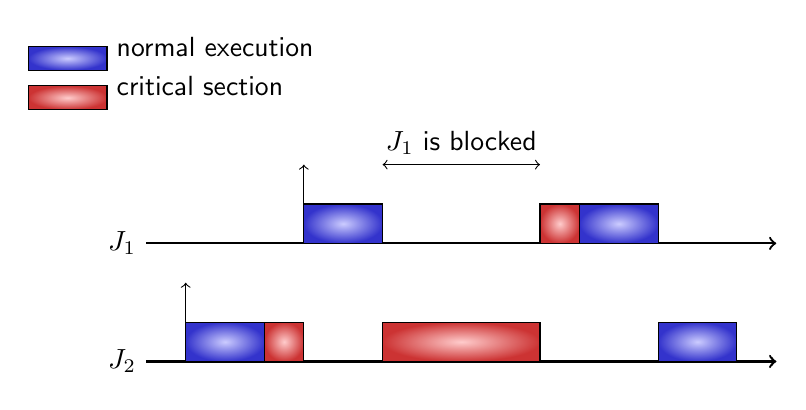
\begin{tikzpicture}[font=\sffamily]
    \begin{scope}[shift={(0,3.2)}]
      \draw[task3](0.5,0) rectangle (1.5, 0.3) node[anchor=west]{critical section};
      \draw[task5](0.5,0.5) rectangle (1.5, 0.8) node[anchor=west]{normal execution};
    \end{scope}
    \draw[->, thick] (2,0) node[anchor=east]{$J_2$} -- (10,0);
    \draw[->](2,0) -- (10, 0);
    \draw[->](2.5,0) -- (2.5, 1);
    \draw[task5](2.5,0) rectangle (3.5, 0.5);
    \draw[task3](3.5,0) rectangle (4, 0.5);
    \draw[task3](5,0) rectangle (7, 0.5);
    \draw[task5](8.5,0) rectangle (9.5, 0.5);
    \draw[->, thick] (2,1.5) node[anchor=east]{$J_1$} -- (10,1.5);
    \draw[->](4,1.5) -- (4,2.5);
    \draw[task5](4,1.5) rectangle (5, 2);
    \draw[task3](7,1.5) rectangle (7.5, 2);
    \draw[task5](7.5,1.5) rectangle (8.5, 2);
    \draw[<->](5,2.5) -- (6, 2.5) node[anchor=south]{$J_1$ is blocked} -- (7, 2.5);
  \end{tikzpicture}
  \end{center}

\end{frame}

\begin{frame}
  \frametitle{Priority Inheritance Protocol (PIP)}

  When a lower-priority job $J_j$ blocks a higher-priority job, the
  priority of job $J_j$ is \emph{promoted} to the priority level of
  highest-priority job that job $J_j$ blocks.

  \vskip 0.2in
    For example, if the priority order is $J_1 > J_2 > J_3 > J_4 > J_5$,
    \begin{itemize}
    \item When job $J_4$ blocks jobs $J_2$ and $J_3$, the priority of
      $J_4$ is promoted to the priority level of $J_2$.
    \item When job $J_5$ blocks jobs $J_1$ and $J_3$, the priority of
      $J_5$ is promoted to the priority level of $J_1$.
    \end{itemize}
\end{frame}



\begin{frame}
\frametitle{Exercises (10 points)}
\begin{enumerate}
\item Please build the source code and execute SEMAPHORE\_TEST example. Then, draw the diagram to check the system behaviours. (3 points)
\item Remove the marked thread\_raise\_priority() in coremutexseize.c to recover PIP behaviours and draw the timing diagram. (2 points)
\item Revise PIP to promote the priority of resource holder to the highest priority. What is the drawback? Please explain in the diagram. (5 points)
\newline Hint: coremutexseize.c, taskcreate.c, find . -type f | xargs fgrep "XXX" 
\end{enumerate}
\end{frame}

\end{document}
